\documentclass{standalone}
\usepackage{pgfplots}
\pgfplotsset{compat=newest}

\begin{document}
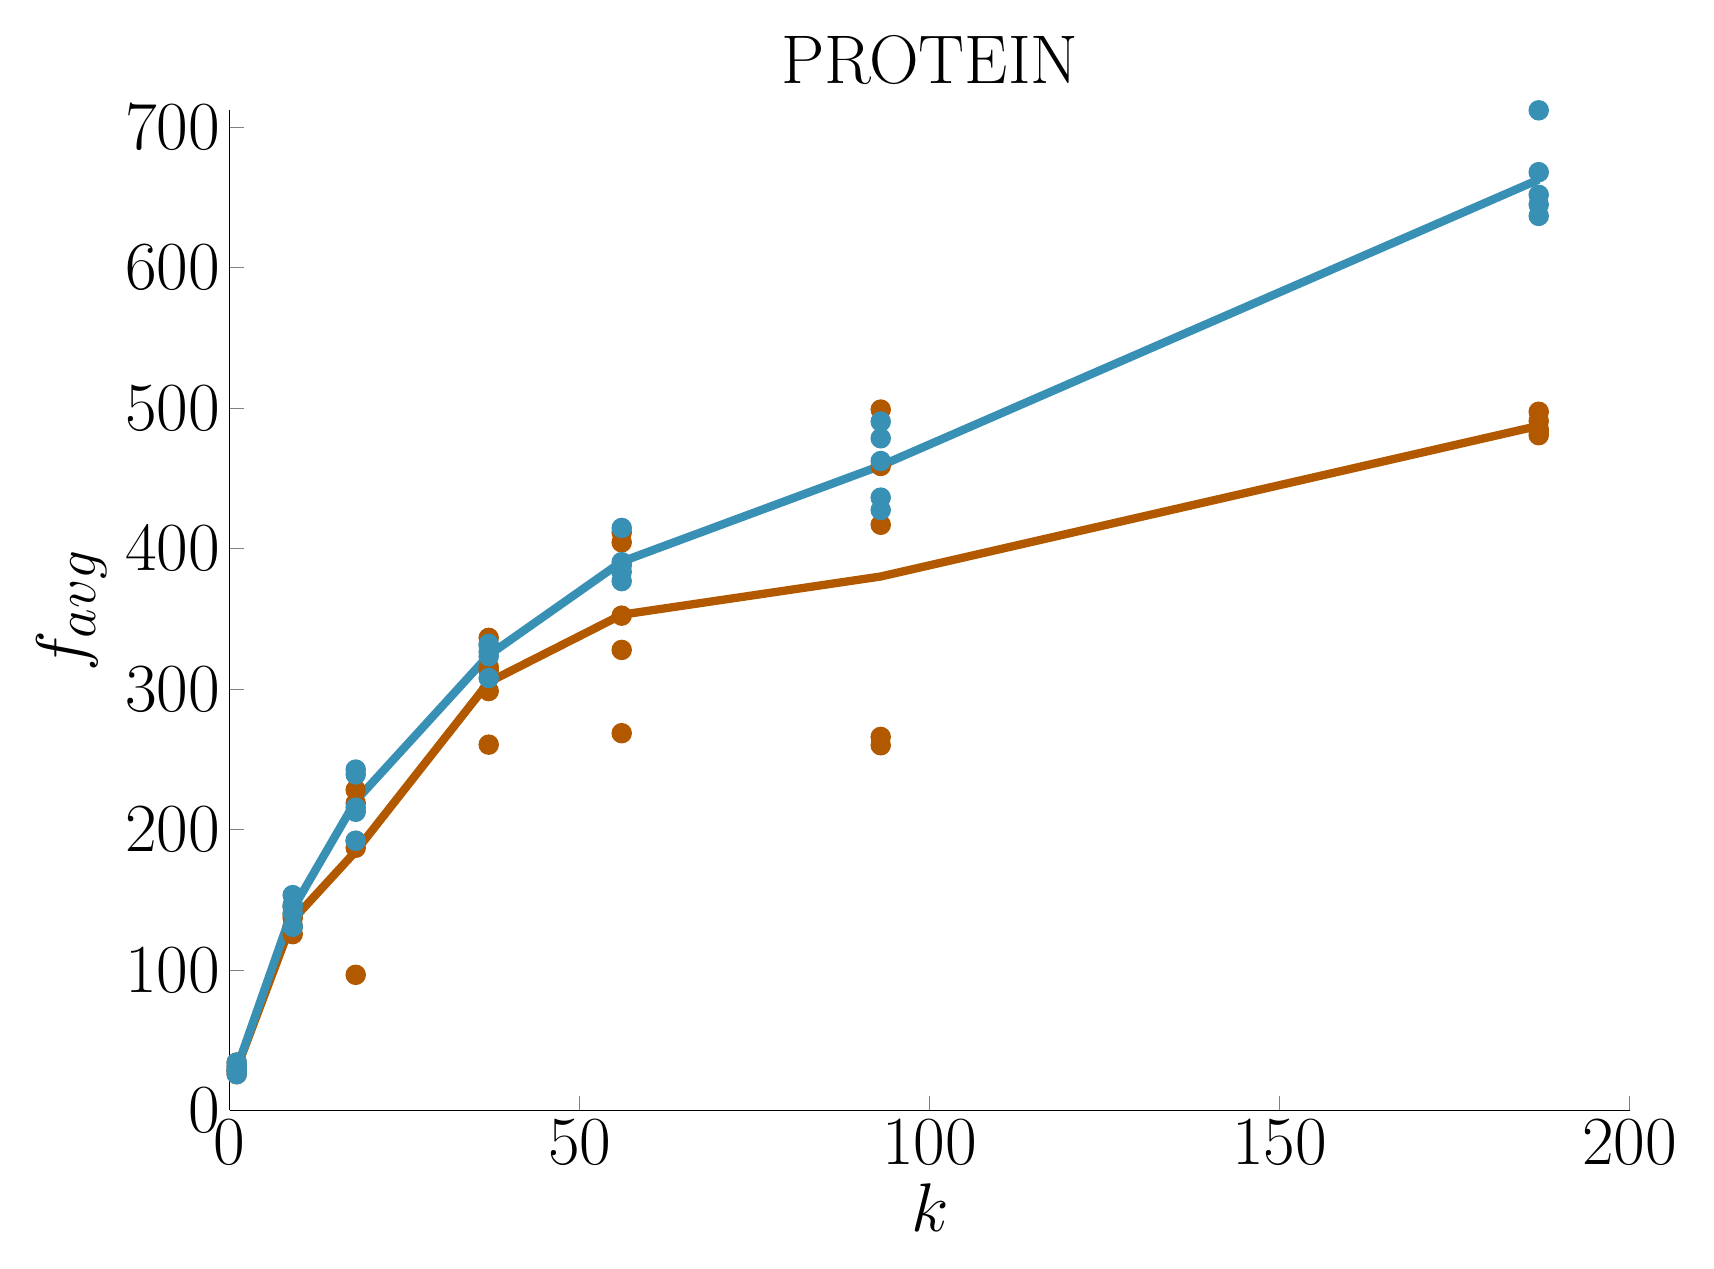
\begin{tikzpicture}

\begin{axis}[%
title style={font=\Huge},
title=PROTEIN,
tick label style={font=\Huge},
label style={font=\Huge},
legend style={font=\Huge},
view={0}{90},
max space between ticks=50pt,
width=7in,
height=5in,
scale only axis,
xmin=0, xmax=200,
xtick={0, 50, 100, 150, 200},
xlabel={$k$},
ymin=0, ymax=712.1,
%ytick={0, 200, 400, 600, 800, 1000},
ylabel={$f_{avg}$},
major tick length=5pt,
axis lines*=left,
legend cell align=left,
clip=false]

\addplot [
only marks,
mark=*,
mark size=3.5pt,
color=orange!70!black,
%solid,
%line width=2pt,
]
coordinates{
(1,25.75)(1,28.5)(1,28.5)(1,31.25)(1,34.0)(9,125.45)(9,131.2)(9,137.0)(9,139.2)(9,144.8)(18,96.5)(18,186.95)(18,191.9)(18,218.7)(18,228.15)(37,260.4)(37,298.55)(37,313.35)(37,315.7)(37,336.45)(56,268.55)(56,327.85)(56,352.25)(56,404.45)(56,411.5)(93,259.95)(93,265.9)(93,416.95)(93,458.85)(93,499.0)(187,480.75)(187,483.2)(187,485.0)(187,490.8)(187,497.45)
};

\addplot [
only marks,
mark=*,
mark size=3.5pt,
color=cyan!70!black,
%solid,
%line width=2pt,
]
coordinates{
(1,25.75)(1,28.5)(1,28.5)(1,31.25)(1,34.0)(9,130.7)(9,140.5)(9,145.35)(9,146.2)(9,153.25)(18,191.95)(18,212.6)(18,215.55)(18,239.15)(18,242.65)(37,307.8)(37,323.35)(37,326.45)(37,330.85)(37,332.1)(56,376.85)(56,383.4)(56,388.15)(56,390.35)(56,414.7)(93,427.5)(93,436.3)(93,462.35)(93,478.55)(93,490.45)(187,636.9)(187,644.95)(187,651.9)(187,668.05)(187,712.1)
};

\addplot [
color=orange!70!black,
solid,
line width=3pt
]
coordinates{
(1,29.6)(9,135.53)(18,184.44)(37,304.89)(56,352.92)(93,380.13)(187,487.44)
};

\addplot [
color=cyan!70!black,
solid,
line width=3pt
]
coordinates{
(1,29.6)(9,143.2)(18,220.38)(37,324.11)(56,390.69)(93,459.03)(187,662.78)
};


\end{axis}
\end{tikzpicture}
\end{document}
